\documentclass[12pt]{article}
\usepackage[latin1]{inputenc}
\usepackage{fancyhdr}
\usepackage{geometry}
\usepackage{makeidx}
\usepackage{graphicx}
\usepackage{epigraph}

\geometry{left=2.5cm,right=2.5cm,top=2.5cm,bottom=3cm}


\title{%
		\begin{Huge}Progetto di Web Information Management\end{Huge} \\
		\begin{Large}
		Analisi di usabilit\'a di un sito
		\end{Large}
}
\date{\vspace{-2ex}}
%\author{Cristian Pirlog}

% Turn on the style
\pagestyle{fancyplain}

% Clear the header and footer
\fancyhead{}
\fancyfoot{}

% Set the footer
\fancyfoot[L]{Cristian Pirlog}
\fancyfoot[R]{\thepage}


% All the text
\begin{document}
\maketitle
\vspace{40ex}

\noindent Sito: \texttt{https://www.goodreads.com}\\

\noindent Author: \textit{Cristian Pirlog}\\
\noindent Matricola: \textit{1097011}\\
\noindent Periodo analisi: \textit{Maggio 2017}
\newpage

\tableofcontents
\newpage

\section{Analisi Preliminare}
Goodreads \'e il sito pi\'u grande al mondo per lettori e raccomandazioni di libri, creato dallo sviluppatore di software ed imprenditore americano Otis Chandler. Il 28 Marzo del 2013, Amazon annunci\'o di aver acquistato Goodreads per 150 Milioni di dollari. \\
Il sito permette agli utenti di cercare gratuitamente all' interno del database di Goodreads libri, recensioni e note. Gli utenti possono registrarsi e aggiungere a loro volta libri per generare cataloghi di librerie e liste di lettura. Inoltre, possono anche creare propri gruppi di suggerimenti di lettura, sondaggi, blog e discussioni. \\
Add oggi Goodreads conta pi\'u di 55 milioni di iscritti e oltre 1.5 Miliardi di libri aggiunti.

\subsection{Struttura}
Goodreads \'e uno social network strutturato in modo tale da permettere a chiunque di vedere i libri contenuti negli scaffali degli amici e le recensioni che questi ultimi hanno lasciato sulla loro bacheca.\\
\\Il sito dispone di un men\'u a sinistra con diverse voci \textbf{(Figure 1)}, tra le quali \textbf{Browser} e \textbf{Community}.
\begin{itemize}
\item Selezionando il primo, si ha accesso ad una lista di categorie che permettono di \textit{trovare raccomandazioni per i prossimi libri da leggere, libri premiati, giveaways, nuovi rilasci oppure semplicemente esplorare l'enorme database a disposizione}.
\item Selezionando invece Community si ha la possibilit\'a di accedere a diverse features presenti nel sito, quali\textit{ i gruppi, le discussioni, i quiz o gli eventi.} E' inoltre possibile \textit{fare delle domande agli autori pi\'u in voga del momento}.
\end{itemize}
Da questo men\'u si ha anche la possibilit\'a di accedere alla propria libreria, selezionando \textbf{My Books}. Qui si potranno anche vedere i diversi scaffali personalmente creati e riempiti. \\ \\
In alto a destra invece c'\'e un men\'u dove si pu\'o selezionare tra diverse opzioni quali notifiche, discussioni all'interno dei gruppi, messaggi, amici o informazioni del proprio profilo.
\begin{figure}
	\centering 
	
\includegraphics[width=16.5cm]{resources/headerbar.png}
	\caption{\textbf{La foto dell'header una volta loggati.}}
\end{figure}
Al centro dell'header invece, troviamo una bara di ricerca, il cui funzionamento approfondiremo pi\'u avanti.
\newpage

\begin{figure}
\section{Homepage:Le 6 W}
\begin{flushleft}
Al primissimo accesso su Goodreads quello che si visualizzer\'a sar\'a ci\'o che verr\'a rappresentato dalla figura seguente: 
\end{flushleft}
	\centering 
	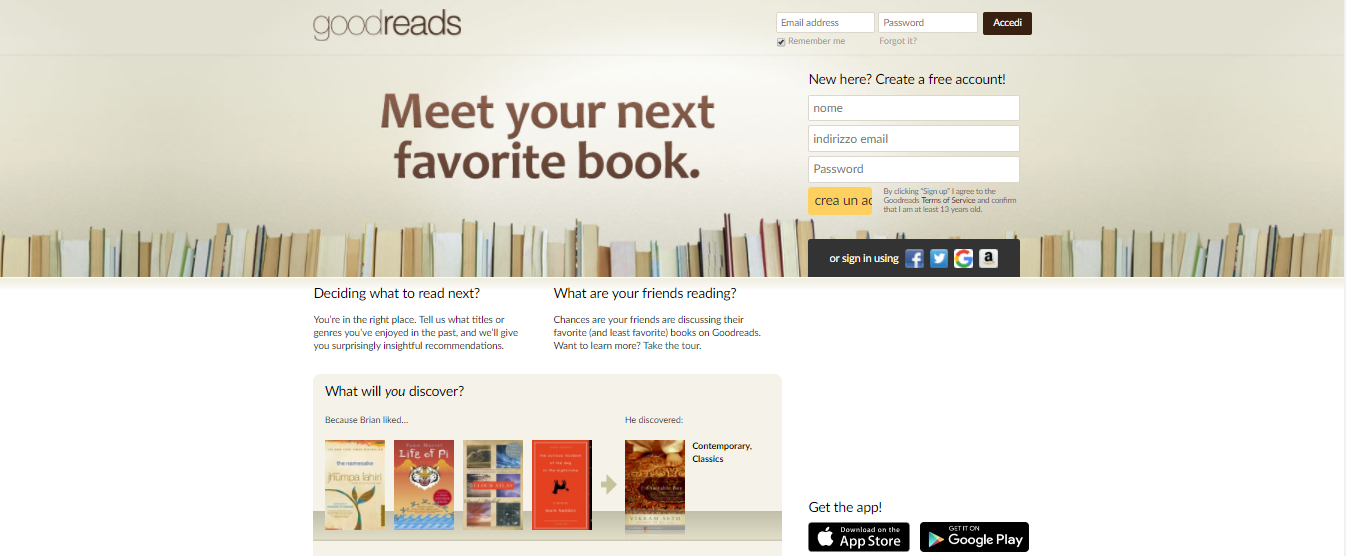
\includegraphics[width=16.5cm]{resources/homenotlogged_1.png}
	\caption{\textbf{Parte superiore della Homepage per un utente non registrato.}}
\end{figure}

\begin{flushleft}
Come si pu\'o notare dalla foto, si ha la possibilit\'a di fare diverse scelte:
\begin{enumerate}
	\item Registrarsi velocemente inserendo poche informazioni oppure collegando il proprio account di Facebook o Twitter, Google, Amazon. Questa molteplicit\'a di scelte spinge l'utente a registrarsi senza preoccuparsi di perdere troppo tempo nel compilare decine di campi. \\
	Un problema invece ben visibile \'e dato dalla localizzazione del sito in italiano. Nello specifico, il pulsante che dovrebbe servire per fare la Submit del form di registrazione contiene il testo 'crea un account' che per\'o non \'e mostrato interamente, date le ridotte dimensioni del pulsante. Un'altra pecca che si pu\'o notare \'e la capitalizzazione delle lettere dei placeholder all'interno dei tag di input e del pulsante sopra citato, la quale sembra essere stata fatta senza un criterio preciso.

	\item Loggarsi inserendo la propria e-mail e password ed avere pieno accesso al contenuto del sito.
	
	\item Informarsi sul contenuto del sito grazie ad una frase ad effetto (\textbf{Meet your next favorite book.}) che fa capire immediatamente all'utente cosa riuscir\'a a trovare, in questo caso il suo prossimo libro preferito.\\
	Ci sono inoltre anche altre informazioni che aiutano l'utente estraneo al sito a capire cosa potr\'a trovare al suo interno come ad esempio i due paragrafi titolati \textbf{Deciding what to read next?} e \textbf{What are your friends reading?}. \textbf{(Figure 2)}
	
	\item Scorrere la pagina per conoscere altre informazioni riguardo al sito. \textbf{(Figure 3)}
	
	\item Nella seconda parte della Homepage \textbf{(Figure3)}, si potranno cercare informazioni all'interno del database di Goodreads anche se non si \'e  loggati.
\end{enumerate}

\end{flushleft}

\begin{figure}
	\centering 
	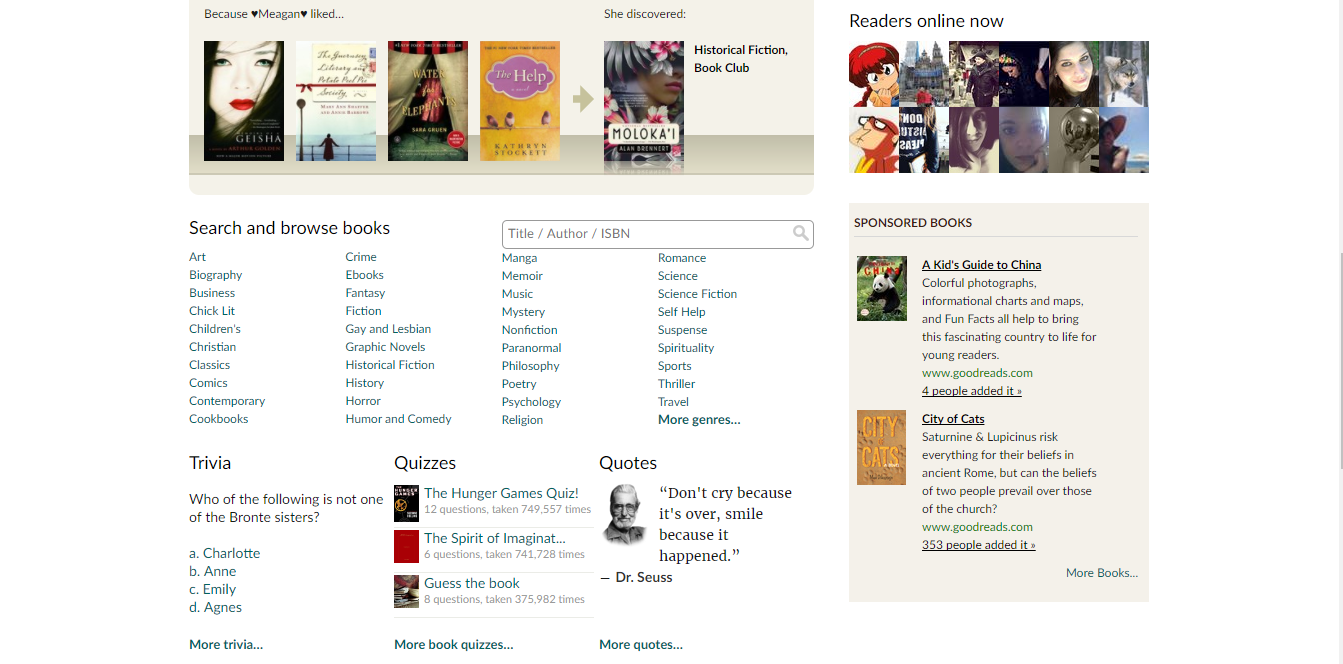
\includegraphics[width=16.5cm]{resources/homenotlogged_2.png}
	\caption{\textbf{Parte centrale della Homepage per un utente non loggato.}}
\end{figure}

{\large \textit{Dato che la gran parte delle funzionalit\'a del sito possono essere sfruttate solo se si \'e loggati, da ora in poi tratteremo solo questa sezione del sito.}}

\subsection{Where?}
\begin{center}
{\large \textit{"A che tipo di sito sono arrivato? Quale contenuto mi offre?"}}
\end{center}



\subsection{Who?}
\begin{center}
{\large \textit{"Chi rappresenta il sito?"}}
\end{center}

\subsection{Why?}
\begin{center}
{\large \textit{"Perch\'e mai dovrei fermarmi su questo sito? Quali benifici mi porta?"}}
\end{center}

\subsection{What?}
\begin{center}
{\large \textit{"Cosa offre il sito?"}}
\end{center}

\subsection{When?}
\begin{center}
{\large \textit{"Quali sono le ultime novit\'a presenti nel sito?"}}
\end{center}


\subsection{How?}
\begin{center}
{\large \textit{"In che modo si arriva alle sezioni principali del sito?"}}
\end{center}




\end{document}
